% !TEX root = ../../document.tex

\documentclass{subfiles}

\begin{document}

  \chapter{Implementación, Resultados y Trabajo Futuro}
  \label{chap:implementation}

    \section{Introducción}
    \label{sec:implementation_intro}

      \paragraph{}
      A lo largo de este documento se han descrito distintas ideas relacionadas con nuevas técnicas para tratar de hacer frente al problema de la complejidad derivada del tamaño de conjunto de datos de tamaño masivo, para el cual es necesario utilizar técnicas sofisticadas que agilicen dichos procedimientos. Dichos conceptos se han descrito desde una perspectiva teórica dejando de lado cuestiones de implementación u otros factores. Dicha abstracción ha permitido simplificar las descripciones teniendo en cuenta únicamente el enfoque algoritmico de las mismas.

      \paragraph{}
      Sin embargo, el enfoque que se seguirá en este capítulo pretende ser muy diferente, centrandose en los detalles de implementación y dejando de lado el contenido matemático. De esta manera, se pretende describir el código fuente desarrollado desde la perspectiva de su estructura y organización, ya que a pesar de basarse en una implementación que trata de ejemplificar conceptos descritos a lo largo del documento, se ha dedicado especial cuidado tratando de escribir código de calidad, mantenible y reutilizable.

      \paragraph{}
      Antes de profundizar en detalles relacionados con la implementación en si, es necesario realizar una explicación acerca de lo que se ha pretendido conseguir mediante el desarrollo de la misma, ya que debido al contexto en que se enmarca (\emph{Trabajo de Fin de Grado} de \emph{Ingeniería Informática}) y la metodología seguida para la realización  del mismo (\emph{Proyecto de Investigación}), esta implementación se encuentra en las primeras fases de su desarrollo, por lo cual aún no tiene el grado de madurez esperado para ser incluida en entornos de producción. A pesar de ello, se cree que la continuación en el desarrollo de la misma es una tarea interesante, que con las horas de trabajo necesarias, se podría convertir en una herramienta interesante frente a otras alternativas que existen actualmente.

      \paragraph{}
      Para entender lo que se ha pretendido conseguir con esta implementación, a continuación se ejemplifica un caso de una implementación similar que se ha llevado a cabo utilizando otras tecnologías en los últimos años. Dicha implementación (e ideas) se conoce como \emph{GraphX}, una biblioteca para el tratamiento de grafos masivos de manera distribuida presentada en \emph{2013} en el trabajo \emph{Graphx: A resilient distributed graph system on spark} \cite{xin2013graphx} desarrollado por \emph{Xin y otros}. Esta implementación se desarrolló inicialmente como un conjunto de utilidades y procedimientos sencillos para facilitar la representación de grafos y el desarrollo de algoritmos sobre estos.

      \paragraph{}
      \emph{GraphX} se ha desarrollado utilizando como base la plataforma de computación distribuida \emph{Spark} publicada en el trabajo \emph{Spark: Cluster computing with working sets} \cite{zaharia2010spark} de \emph{Zaharia y otros}. Esta plataforma se basa en el tratamiento de grandes conjuntos de datos mediante el procesamiento de los mismos en lotes, lo cual proporciona grandes mejoras respecto de otras soluciones como \emph{Hadoop}, presentado en el documento \emph{The hadoop distributed file system} \cite{shvachko2010hadoop} desarrollado por \emph{Shvachko y otros}.

      \paragraph{}
      Dichas plataformas tratan de abstraer la idea de procesamiento distribuido y hacerlo lo más transparente posible para el usuario, sin olvidar en ningún momento que los conjuntos de datos utilizados sobre los que se trabaja no se encuentran contenidos totalmente en una única máquina, lo cual implica distintas restricciones respecto de las estrategias de programación clásicas, como los procesos de acceso y escritura al sistema de almacenamiento. Sin embargo, en estos casos también existen soluciones que abstraen dichas tareas de almacenamiento distribuidas, algunas de ellas son \emph{Google File System} \cite{ghemawat2003google} o \emph{Hadoop File System} \cite{shvachko2010hadoop}.

      \paragraph{}
      Lo característico de \emph{GraphX} es que se ha desarrollado como una biblioteca para el tratamiento de grafos utilizando \emph{Spark} como plataforma base, pero tratando de mantener la independencia entre las mismas. Es decir, \emph{GraphX} ha sido desarrollado utilizando las utilidades que proporciona \emph{Spark}, pero en \emph{Spark} no existe ninguna dependencia hacia \emph{GraphX}. Por tanto, esto se puede entender como un sistema basado en capas, donde \emph{Spark} representa la capa inferior y \emph{GraphX} se coloca en una capa inmediatamente superior.

      \paragraph{}
      En este trabajo, se ha tratado de realizar una implementación semejante (a un nivel muy básico por las restricciones temporales en que se ha desarrollado), tratando de proporcionar igualmente una capa de abstracción que modeliza el concepto de grafo sobre otra plataforma de computación de alto rendimiento. En este caso se ha decidido utilizar la biblioteca de cálculo intensivo \emph{TensorFlow}, la cual se hizo pública en \emph{2016} en el trabajo \emph{Tensorflow: Large-scale machine learning on heterogeneous distributed systems} \cite{abadi2016tensorflow}, desarrollada por el departamente de investigación de \emph{Google} y actualmente publicada con licenciatura de código abierto.

      \paragraph{}
      \emph{TensorFlow} proporciona un \emph{framework} para la implementación de algoritmos cuyo funcionamiento se basa en el cálculo de operaciones sobre \emph{tensores} (una generalización del concepto de matriz). Se ha preferido posponer la descripción de esta plataforma hasta la sección \ref{sec:tensorflow}, ya que a continuación se describirá el conjunto de tecnologías utilizadas para la implementación realizada.

      \paragraph{}
      La motivación por la cual se ha decidido realizar la implementación de una biblioteca que simplifique el desarrollo de algoritmos sobre grafos utilizando una plataforma de cálculo matemático intensivo se debe a lo siguiente: una gran cantidad de analíticas sobre grafos pueden ser calculadas entendiendo dicho grafo como una estructura de datos matricial, a través de la \emph{matriz de adjacencia} (sección \ref{sec:adjacency_matrix}), u otras representaciones como la \emph{matriz laplaciana} (sección \ref{sec:laplacian_matrix}). Este marco conceptual conlleva el desarrollo de algoritmos con un alto grado de paralelización, que tal y como se verá posteriormete, satisface la plataforma \emph{TensorFlow}.

      \paragraph{}
      Sobre este contexto también se pueden desarrollar algoritmos de optimización, tales como planificación de rutas, recorridos de vehículos o cubrimiento de zonas mediante la modelización del grafo de manera conveniente y la utilización de distintas estrategias de programación lineal, lo cual se ha estudiado ampliamente en la literatura.

      \paragraph{}
      En este caso, la implementación realizada para este trabajo se encuentra en las primeras fases de su desarrollo. Por tanto, únicamente se ha basado en el conjunto de utilidades necesarias para llevar a cabo la implementación del \emph{Algoritmo PageRank} (capítulo \ref{chap:pagerank}), junto con un \emph{Sparsifier} (sección \ref{sec:sparsifiers}) que reduce el número de aristas del grafo para después comparar resultados a nivel de precisión.

      \paragraph{}
      Sin embargo, tal y como se indicará posteriormente, se pretende seguir trabajando en dicha biblioteca de grafos para ampliar su funcionalidad y desarrollar otras implementaciones que permitan obtener otras analíticas sobre el grafo.

      \paragraph{}
      El resto del capítulo se organiza de la siguiente manera: en la sección \ref{sec:implementation} se realiza una descripción acerca de las decisiones tomadas en la implementación de la biblioteca, indicando las tecnologías utilizadas (sección \ref{sec:used_technologies}), los servicios en que se ha apoyado el desarrollo (sección \ref{sec:used_services}) y el diseño que ha seguido dicha implementación (sección \ref{sec:implementation_design}). Posteriormente se realiza un comentario acerca de los resultados obtenidos en la sección \ref{sec:implementation_results}. A continuación se indican distintas vías a través de las cuales sería interesante seguir trabajando en la implementación en la sección \ref{sec:future_work} y, por último, se realiza una breve conclusión acerca del trabajo realizado en la sección \ref{sec:implementation_conclusions}

    \section{Implementación}
    \label{sec:implementation}

      \paragraph{}
      En esta sección se exponen distintas explicaciones acerca de la implementación realizada, la cual pretende comportarse como una biblioteca de utilidades que permita modelizar de manera sencilla el concepto de grafo, utilizando como base una plataforma de cálculo matemático intensivo. Dicha implementación se ha realizado prestando especial atención en la reducción de dependencias hacia el exterior, de tal manera que sea posible la distribución de la misma como un paquete compacto que integrar en otros sistemas de mayor envergadura. Por tanto, se ha utilizado el sistema de distribución de paquetes del lenguaje \emph{Python}, el cual simplifica dicha tarea. Sin embargo, antes de comenzar a describir distintos detalles acerca de las decisiones tomadas, a continuación se describen brevemente las tecnologias utilizadas, ya que son influyentes respecto de dichas decisiones.

      \subsection{Tecnologías Utilizadas}
      \label{sec:used_technologies}

        \paragraph{}
        La implementación se ha desarrollado utilizando el lenguaje \emph{Python}, junto con distintas bibliotecas que extienden su comportamiento y le otorgan una mayor funcionalidad. Además, se ha utilizado el sistema de control de versiones \emph{git}, que permite trabajar de manera ordenada en distintas partes del trabajo.

        \subsubsection{Python}
        \label{sec:python}

          \paragraph{}
          \emph{Python} se define como un lenguaje de propósito general sobre un paradigma imperativo pero con utilidades de programación funcional como funciones lambda o tratamiento de funciones como un valor más. Es orientado a objetos y no tipado, lo cual simplifica el trabajo a la hora de escribir código, pero limita la seguridad del mismo ante entradas incorrectas. Python es un lenguaje interpretado en tiempo de ejecución, por lo cual no es requiere de la utilización de un compilador. Internamente existen implementaciones de \emph{Python} en distintos lenguajes de programación compilados, sin embargo, en este caso el desarrollo se ha realizado sobre \emph{cpython}, que se basa en un itérprete desarrollado en el lenguaje \emph{C}.

          \paragraph{}
          En la revisión del estándar \emph{PEP-484} \url{https://www.python.org/dev/peps/pep-0484/} se añade un sistema de marcado de tipos para el lenguaje, el cual aún no está operativo en tiempo de ejecución (a través del intérprete), pero permite la comprobación estática del mismo. En la implementación realizado se ha utilizado este este sistema de comprobación de tipos, el cual se introdujo en \emph{Python 3.5}, por tanto está ha sido la versión escogida como mínima.

          \paragraph{}
          \emph{Python} implementa como estructura de datos indexadas \emph{listas enlazadas}, lo cual proporciona una gran versatilidad ya que permite tanto agregrar como eliminar nuevos elementos de manera eficiente ($O(1)$). Sin embargo, el tiempo de acceso se ve altamente penalizado por dicha condición ($O(n)$). Por tanto, se han utilizado bibliotecas externas que mejoran dichos costes.

        \subsubsection{NumPy y Pandas}
        \label{sec:numpy_pandas}

          \paragraph{}
          Para solventar la problemática de la eficiencia en tiempo de acceso de las estructuras de datos indexadas en \emph{Python} existe una biblioteca que permite implementa dichas estructuras de datos de manera contigua, lo cual elimina el problema. Dicha biblioteca se conoce como \emph{NumPy} \cite{walt2011numpy}, la cual proporciona además un gran conjunto de operaciones matemáticas sobre esta estructura de datos. De esta manera se permite desarrollar algoritmos con una elevada carga matemática de manera muy eficiente y a la vez sencilla, al estilo de lenguajes como \emph{MatLab} o \emph{R}.

          \paragraph{}
          Para algunas partes del código implementado, se ha utilizado la biblioteca \emph{Pandas} \cite{mckinney2010data}. Esta biblioteca consiste en una extensión respecto de \emph{NumPy}, que permite ver la estructura de datos desde una perspectiva de conjunto de datos en lugar de estructura matemática, lo cual simplifica el trabajo para tareas como la lectura y estructa de conjuntos de datos en el espacio de almacenamiento.

        \subsubsection{TensorFlow}
        \label{sec:tensorflow}

          \paragraph{}
          \emph{TensorFlow} \cite{abadi2016tensorflow} es una biblioteca inicialmente desarrollada por \emph{Google}. La idea principal por la cual fue desarrollada es la simplificación de tareas para la implementación de algoritmos para aprendizaje automático y \emph{deep learning}, cuya carga computacional es altamente paralelizable y puede ser entendida como operaciones entre \emph{tensores}. Esta biblioteca proporciona interfaces para ser utilizada junto con los lenguajes \emph{Python}, \emph{C++}, \emph{Java} o \emph{Go}.

          \paragraph{}
          Un \emph{tensor} es una generalización del concepto de matriz, permitiendo que estas sean de cualquier número de dimensiones. Esto puede entenderse fácilmente diciendo que un tensor de grado 0 se corresponde con el concepto de escalar, uno de grado 1 puede ser visto como un vector, el grado 2 se corresponde con las matrices y así sucesivamente. A partir del conjunto de operaciones aplicable a dichos \emph{tensores} se crea un flujo de estas, que puede ser visto como un grafo de dependencias entre ellas. Por tanto, el la biblioteca se decidió llamar \emph{TensorFlow} (\emph{flujo de tensores}).

          \paragraph{}
          \emph{TensorFlow} proporciona por tanto, estructuras de datos para representar el concepto de \emph{tensor} así como un conjunto de operaciones básicas que aplicar entre ellos para así obtener nuevos \emph{tensores} con los resultados. La biblioteca se puede dividir en dos bloques bien diferenciados: el primero de ellos de bajo nivel y que se corresponde con operaciones matemáticas sencillas (suma, multiplicacion, division, exponenciación, máximos, etc.) y otro segundo bloque construido a partir del primero al cual pertenece todo el conjunto de operaciones de alto nivel que permiten la implementación de algoritmos de aprendizaje automático fácilmente, tales como implemenentaciones del \emph{gradiente descendente} u otros conceptos semejantes. Independientemente de estos dos bloques, la biblioteca también proporciona otra serie de utilidades como capacidad para definir variables y constantes, guardar y recuperar modelos matemáticos y otras facilidades.

          \paragraph{}
          En esta implementación se han utilizado métodos relacionados con operaciones algebraicas, ya que se ha utilizado dicha libreria centrandose únicamente en su perspectiva matemática y obviando por completo el bloque de aprendizaje automático, ya que no se corresponde con el tema de este trabajo ni con las ideas descritas en anteriores capítulos.

          \paragraph{}
          \emph{TensorFlow} proporciona distintas ventajas a nivel de rendimiento respecto de otras alternativas de computación numérica intensiva puesto que está construida como una interfaz de alto nivel que abstrae al usuario del sistema donde está siendo ejecutado el cómputo. Con esto nos estamos refiriendo a que la implementación realizada es ejecutable tanto en una \emph{CPU} clásica de un ordenador como en acelerados de computación externos tales como \emph{GPU's} \emph{CUDA} o las \emph{Tensor Processor Units} \cite{jouppi2017datacenter} diseñadas expecificamente por \emph{Google} para ser utilizadas junto con esta librería.

          \paragraph{}
          Debido a estas ideas, el estilo de programación se divide en dos fases, una de definicion de tensores, operaciones y relaciones de dependencia entre ellas en la cual se construye el denominado flujo o grafo de operaciones, y una segunda fase correspondiente a la llamada para la ejecución de dichas operaciones. Esta idea cobra sentido debido tanto al elevado tamaño de los datos de entrada para las operaciones, así como el modelo de computación en aceleradores externos, que requiere de tareas de transferencia entre el sistema y dichas unidades. Al dividirse la definición de la ejecución, esto se puede optimizar de manera eficiente sobre lenguajes interpretados como \emph{Python}, que sino tendrían una alta penalización en temporal derivada del coste de transferencias.

        \subsubsection{pytest}
        \label{sec:tensorflow}

          \paragraph{}
          \emph{pytest} es una herramienta de generación de casos de prueba para el lenguaje \emph{Python}. Para ello se basa en la ejecución de distintas funciones definidas por el usuario, las cuales contienen un conjunto de asertos (palabra reservada \emph{assert} en \emph{Python}), los cuales deben superar satisfactoriamente para finalizar el test de manera satisfactoria. Para los casos de prueba, estos se han utilizado junto con los que proporciona \emph{NumPy} para comprobar la semejanza entre dichas estructuras de datos de manera eficiente.

        \subsubsection{sphinx}
        \label{sec:sphinx}

          \paragraph{}
          \emph{sphinx} consiste en una herramienta que permite extraer la documentación incorporada en el código a otras fuentes para facilitar su visualización, tales como un sitio web, documentos de \emph{PDF} y otras alternativas. Para ello se basa en la documentación interna del código. En el caso de \emph{Python}, esta documentación se denomina \emph{docstring} y permite añadir una breve explicación acerca de los bloques de código, así como las entradas y salidas de los métodos. En este caso se ha utilizado el estilo de documentación definido por \emph{Google} para tratar de asemejarse lo máximo posible a la documentación seguida por \emph{TensorFlow}

        \subsubsection{git}
        \label{sec:git}

          \paragraph{}
          \emph{git} se corresponde con un \emph{sistema de control de versiones} que permite el trabajo de manera colaborativa entre distintos usuarios, a través de distintas ramas de desarrollo, que después se combinan para llegar a un estado de desarrollo final. Además de esto, permite almacenar un historial de todos los cambios realizados, lo cual es de gran ayuda en puntos en los cuales es necesario entender la razón de cambios pasados así, como retroceder hasta un estado anterior si fuera conveniente. Otra de las ventajas de esta herramienta es la capacidad de sincronización entre distintos sistemas, así como la posibilidad de mantener una copia del repositorio en un servidor externo, lo cual previene de problemas relacionados con fallos del sistema local.

      \subsection{Servicios Utilizados}
      \label{sec:used_services}

        \paragraph{}
        Para el desarrollo de este trabajo se han utilizado distintos servicios de empresas externas que simplifican algunas de las tareas inherentes en la utilización de las tecnologías descritas anteriormente. Dichas tareas se pueden realizar de manera independiente a estos servicios, sin embargo, resulta interesante su utilización por el grado de mayor confiabilidad que proporcionan respecto del desarrollo completo utilizando únicamente una máquina local, que puede sufrir fallos perdiendo todo el trabajo. Todos los servicios externos utilizados han sido utilizados en su versión gratuita, que ofrece las funcionalidades suficientes para el correcto desarrollo del proyecto.

        \paragraph{GitHub}
        Proporciona un servidor \emph{git} externo sobre el cual se realizan copias del trabajo local de tal manera que se aumenta el grado de seguridad desde el punto de la aparición de pérdidas inesperadas. Además del servicio de control de versiones basado en \emph{git}, se proporcionan otra serie de funcionalidades como gestión de incidencias mediante el concepto de \emph{issue}, la fusión de ramas de manera segura a partir de \emph{pull request} o una gestión de proyectos mediante un tablero \emph{kanban} configurable según las necesidades especificas del mismo.

        \paragraph{Read the Docs}
        Ofrece un servicio de generación y publicación de sitios web basados en la documentación de proyectos sofware basada en \emph{sphinx} de manera sencilla, ya que únicamente requiere de la dirección de acceso al repositorio de trabajo \emph{git} junto con las opciones del entorno de desarrollo necesarias para utilizar \emph{sphinx} sobre dicho repositorio. Se cree conveniente la publicación de la documentación de código para que sea accesible fácilmente, por lo cual se decidió utilizar dicho servicio.

        \paragraph{Travis CI}
        Consiste en un entorno de realización de casos de prueba previamente configurados por el usuario a través de bibliotecas como \emph{pytest} u otras similares. El servicio ejecuta despliega un entorno de pruebas previamente configurado por el usuario para después ejecutar el conjunto de casos de prueba indicados. Este servicio indica tras cada cambio en el repositorio si las pruebas han sido superadas, o por contra han ocurrido fallos, indicando el punto de dichos fallos.

        \paragraph{Codecov}
        Es una utilidad interesante que determina el grado de covertura de los casos de prueba sobre la implementación realizada, lo cual proporciona una buena estimación acerca del conjunto de lineas de código que están siendo verificadas por los tests. Sin embargo, a pesar de que esta utilidad proporciona una buena estimación, su resultado tan solo puede ser orientativo, ya que únicamente tiene en cuenta si existe un caso de prueba que analice una determinada línea de código. Esto no tiene en cuenta casos específicos como divisiones entre cero, verificaciones de valores fuera de rango o casos similares.

        \paragraph{WakaTime}
        Es una utilidad destinada al seguimiento de horas de trabajo, que indica tanto la proporción de tiempo destinada a cada lenguaje como a cada proyecto. Esta se basa en la recolección de información sobre los editores de código. Por tanto, recoge el tiempo de trabajo destinado a dicha tarea. Esto es una métrica interesante, pero no tiene en cuenta la cantidad de tiempo destinado a tareas de aprendizaje e investigación leyendo artículos o leyendo documentación de bibliotecas utilizadas durante el desarrollo.

        \paragraph{}
        Todos estos servicios se han utilizados de manera relacionada entre si, en algunos casos de manera directa, mientras que en otros de manera indirecta. El punto de conexión entre todos ellos es el sistema de control de versiones \emph{git}, que estos utilizan para relacionar la tarea que realizan con un determinado proyecto. El sistema de documentación de \emph{Read the Docs} realiza una nueva ejecución tras cada cambio en el repositorio \emph{git} de \emph{GitHub}. De la misma manera \emph{Travis CI} y \emph{Codecov} realizan sus tareas correspondientes. Por último, \emph{WakaTime} realiza un seguimiento constante sobre el tiempo dedicado al repositorio. De esta manera se obtiene un entorno de trabajo que permite un desarrollo ágil permitiendo al desarrollador centrarse únicamente en las tareas de investigación y desarrollo, para posteriormente validar los resultados de ejecución de estos servicios, lo cual reduce tiempo y costes.

      \subsection{Diseño de la implementación}
      \label{sec:implementation_design}

        \paragraph{}
        [TODO ]

        \paragraph{}
        [TODO hablar de python package]

        \subsubsection{Diagrama de Clases}
        \label{sec:class_diagram}

          \paragraph{}
          [TODO ]

          \begin{figure}
            \centering
            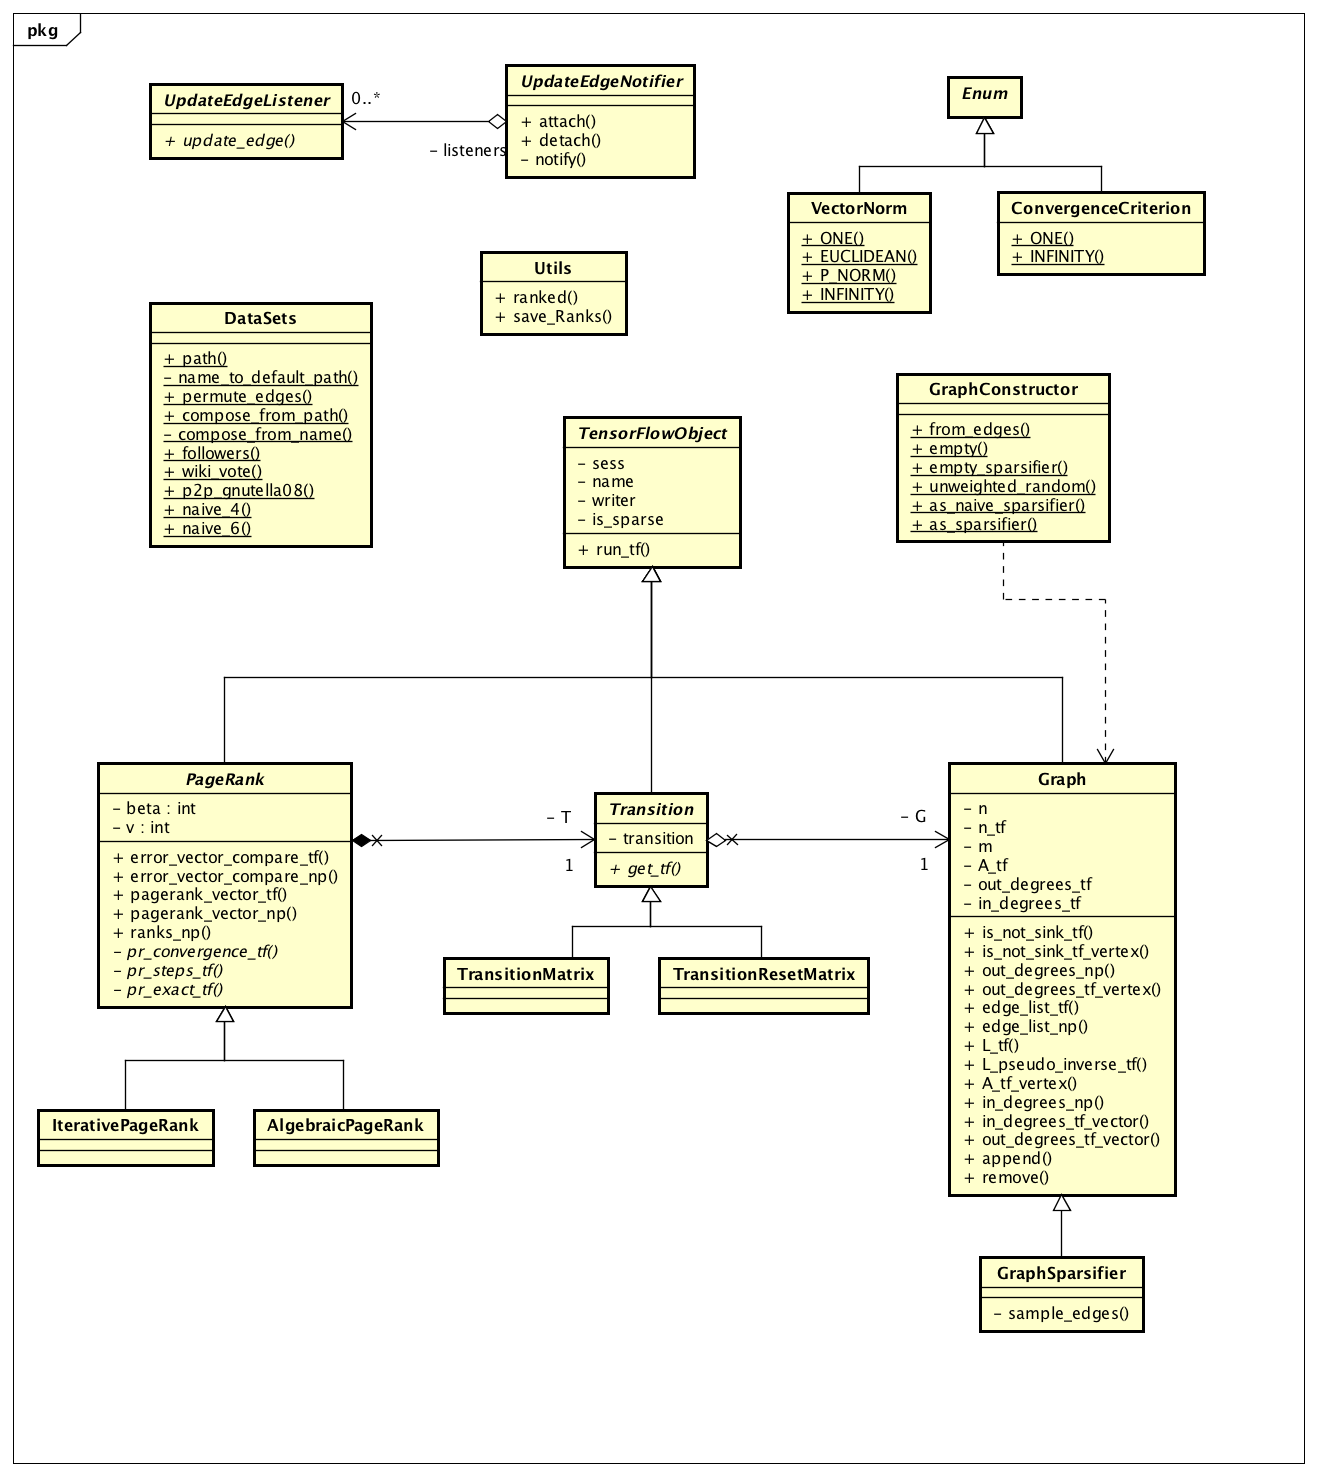
\includegraphics[width=\textwidth,height=\textheight,keepaspectratio]{class-diagram}
            \caption{[TODO ]}
            \label{img:class_diagram}
          \end{figure}


        \subsubsection{Diagrama de Componentes}
        \label{sec:components_diagram}

          \paragraph{}
          [TODO ]

      \paragraph{}
      [TODO]

    \section{Resultados de Implementación}
    \label{sec:implementation_results}

      \paragraph{}
      [TODO]

    \section{Trabajo Futuro}
    \label{sec:future_work}

      \paragraph{}
      El trabajo realizado se puede enmarcar en una zona intermedia entre un trabajo de investigación y un trabajo de implementación práctica, puesto que una gran cantidad del mismo se ha destinado a adquirir nuevos conceptos relacionados con el ámbito del tratamiento de grandes conjuntos de datos. Esto se ve reflejado en los primeros capítulos del trabajo, marcadamente más teóricos que este último, en el cual se indican detalles y razonamientos acerca de las decisiones de implementación.

      \paragraph{}
      Debido al tiempo limitado en la realización del trabajo, así como el contexto académico junto con la compaginación de la realización al mismo tiempo que con otras asignaturas de la titulación, no se ha podido realizar de la manera tan extensa que se hubiera deseado. Además, se cree que el grado de extensión de los conceptos que se describen a lo largo del trabajo así como el proceso iterativo que se puede llevar a cabo para seguir trabajando en la implementación desarrollada lo hacen un trabajo continuable en el futuro.

      \paragraph{}
      Resultaría interesante seguir trabajando en el proyecto de una manera similar, siguiendo un equilibrio equitativo entre las horas de investigación en técnicas para la reducción de la complejidad de grafos de tamaño masivo, junto con la creación de un ecosistema de utilidades que permiten la implementación de estas técnicas así como nuevas métricas como el \emph{conteo de triángulos} u otros algoritmos, aprovechando la implementación inicialmente desarrollada.

      \paragraph{}
      Muchas de estas ideas podrían llegar resultados interesantes en el futuro mediante la realización de un estudio intensivo del problema así como una adecuada base matemática que facilite la comprensión de los trabajos desarrollados por los expertos en la materia, puesto que se cree que en el futuro será necesaria la utilización de técnicas como las estudiadas para hacer frente a los problemas que se están dando en la actualidad, tales como planificación de rutas u otros, que además, continene una componente dinámica muy importante.

      \paragraph{}
      Al igual que en el caso de la investigación, se cree que continuar con el proceso de implementación de una biblioteca de utilidades que permita la implementación y desarrollo de soluciones basadas en grafos sobre una plataforma como \emph{TensorFlow} podría resultar muy interesante, al igual que sucedió con \emph{GraphX} y \emph{Spark}.

      \paragraph{}
      Por tanto, existen distintas lineas de trabajo sobre las cuales poder seguir en este área, todas ellas muy relacionadas entre si, y que podrían llegar a resultados satisfactorios con el correspondiente trabajo y dedicación.

    \section{Conclusiones}
    \label{sec:implementation_conclusions}

      \paragraph{}
      En esta sección se pretende realizar una descripción a nivel de resultados obtenidos tras realizar el \textbf{Trabajo de Fin de Grado} completo. Es decir, tanto la parte de investigación y estudio de \emph{Algoritmos para Big Data}, desde la modelización de \emph{Streaming} (capítulo \ref{chap:streaming}) y las \emph{Estrategias de Sumarización} (cápitulo \ref{chap:summaries}) de información necesarias para agilizar la obtención de resultados sobre conjunto de datos masivos, como las aplicadas a \emph{Grafos} (capítulo \ref{chap:graphs}) y el estudio del algoritmo implementado \emph{PageRank} (capítulo \ref{chap:pagerank}).

      \paragraph{}
      Dichos estudios han permitido conocer de manera más profunda los factores que dificultan la tarea de diseño de algoritmos, cuya ejecución continue siendo factible aún cuando el conjunto de datos crece de manera drástica y es necesario que las consultas sean realizadas en un periodo reducido de tiempo. Esto implica una tarea compleja, para la cual es necesario poseer una extensa base matemática que agilice las tareas de razonamiento y entendimiento acerca de la información encontrada.

      \paragraph{}
      Sin embargo, a pesar de la dificultad propiciada por dicha carga matemática, se ha tratado de hacer frente al trabajo de investigación mediante la lectura de una gran cantidad de artículos científicos en las cuales aparecen explicaciones e ideas muy acertadas. Algo que ha servido para introducirse y conocer cómo es el proceso de investigación, en numerosas ocasiones frustrante y complejo, pero que también ofrece un alto índice de satisfacción personal cuando se consiguen los propósitos alcanzados.

      \paragraph{}
      Desde la perspectiva de los resultados obtenidos a nivel de investigación, estos no han sido satisfactorios desde el punto de vista del describrimiento o análisis de una nueva técnica aplicable sobre el área de investigación que se ha estudiado a lo largo del trabajo. Sin embargo, esto no se entiende como algo totalmente negativo puesto que a través de este proceso se han aprendido una gran cantidad de nuevos conceptos más amplios respecto de los prefijados para un \emph{Graduado en Ingeniería Informática}, los cuales se han creido interesantes y útiles en el futuro.

      \paragraph{}
      La introducción en el ámbito de la investigación, el aprendizaje de distintas estrategias para leer artículos (ya que requieren de práctica y metodología en comparación con otro tipo de literatura), y la gestión del tiempo en dichas tareas han sido un conjunto de conocimientos transversales, que además del aprendizaje inherente relacionado con el \emph{Big Data} se han creido extremadamente útiles para el futuro. Además, el estudio en profundidad de la problemática mediante artículos donde los autores originales de los trabajos exponen sus ideas se ha creido muy enriquecedor para las tareas posteriores de implementación.

      \paragraph{}
      Respecto de los resultados obtenidos desde el punto de vista de la implementación, se ha creido interesante el aprendizaje completo en cuanto al despliegue de un entorno de desarrollo que realice pruebas automatizadas, genere documentación y mantenga un seguimiento acerca de las horas de trabajo, así como la encapsulación de la implementación en un paquete autocontenido de \emph{Python}, distribuible e instalable en otros sistemas es una tarea interesante, que hasta el momento no se había llevado a cabo debido a la rama escogida en los dos últimos años del grado (centrada mayoritariamente en aspectos algorítmicos y computacionales).

      \paragraph{}
      La implementación realizada ha servido para entender en profundidad el algoritmo \emph{PageRank}, así como las ideas subyacentes que permiten entender su procedencia así como su convergencia hacia un resultado satisfactorio. En cuanto a la implementación de los \emph{Sparsifiers}, partir de estos se ha conseguido entender en mayor medida las ventajas y dificultades derivadas de la addición de un grado de indeterminismo sobre un \emph{Grafo}, tratando de perturbar al mínimo posible la estructura del mismo, lo cual es una tarea compleja, pero que se ha creido muy interesante para el futuro.

      \paragraph{}
      El \emph{Trabajo de Fin de Grado} ha servido para comprender el grado de dificultad que representa la realización de un proyecto de mayor envergadura que una práctica de una asignatura del grado, con una fecha prefijada y un periodo relativamente largo de tiempo para su ejecución. En este trabajo se ha tenido muy en cuenta la necesidad de organización y constancia personal diaria para poder asimilar la gran cantidad de conceptos estudiados así como la complejidad de las tecnologías utilizadas para la implementación, que muchas no habían sido utilizadas anteriormente. Esto ha proporcionado un grado de experiencia que se cree favorable y necesario para la finalización de los estudios por un graduado en \emph{Ingeniería Informática}. Sin embargo, este trabajo debe marcar un punto de comienzo sobre el cual mejorar en futuras ocasiones a partir de la experiencia, ya se los errores cometidos durante el desarrollo del mismo no se deben entender como algo negativo, sino como factores que no se deben repetir en futuros proyectos similares.

\end{document}
